\documentclass[a4paper]{article}
\usepackage[utf8]{inputenc}
\usepackage{fullpage}
\usepackage{csquotes}
\usepackage[ngerman]{babel}
\usepackage{biblatex}
\usepackage{float}
\usepackage{graphicx}
\usepackage{epstopdf}
\usepackage{subfigure}
\usepackage[table]{xcolor}
\usepackage[format=plain,labelfont=bf,up]{caption}
\setcounter{secnumdepth}{-1} 
\usepackage{hyperref}
\usepackage{nameref}
\usepackage{minted}
\usemintedstyle{friendly}
\bibliography{paper}
\title{Tenzing \\ A SQL Implementation On The MapReduce Framework}
\author{Willi Schönborn}
\date{\today}
\begin{document}

\begin{figure}[H]
\centering

\includegraphics[width=0.5\textwidth]{beuth.eps}
\maketitle
\end{figure}

\newpage

\tableofcontents

\newpage

\section{Einleitung}
Als Teil der Lehrveranstaltung \textit{Programmierung - Fortgeschrittene Konzepte} im Wintersemester 2011/2012 an der \textit{Beuth Hochschule für Technik Berlin} sollte im Rahmen einer Semesterarbeit ein wissenschaftliches Paper ausgewählt, untersucht und bewertet werden. Das Ziel dieses Dokumentes ist es die Ergebnisse dieser Semesterarbeit zusammenzufassen.

Ausgewählt wurde das Google-Paper \textit{Tenzing A SQL Implementation On The MapReduce Framework} \cite{TENZING}. Erschienen ist das Paper als Teil der Proceedings zur 37th VLDB, der \textit{International Conference on Very Large Data Bases} im September 2011. Die Autoren sind die Google-Mitarbeiter Biswapesh Chattopadhyay, Liang Lin, Weiran Liu, Sagar Mittal, Prathyusha Aragonda, Vera Lychagina, Younghee Kwon und Michael Wong.

\section{Kurzbeschreibung}
Tenzing beschreibt eine SQL92-kompatible Implementierung auf Basis des Google-eigenen MapReduce-Frameworks \cite{MAPREDUCE}. Die beiden grundelegenden Technologien werden in den Kapiteln \textit{\nameref{sql}} und \textit{\nameref{mapreduce}}, unter Berücksichtigung des Hauptthemas, näher erläutert.

\newpage

\section{SQL}
\label{sql}

SQL steht für \textit{Structured Query Language} und ist eine mengenorientierte, deklarative Abfragesprache für Datenbank-Management-Systeme.

Standardisierung

DML
DDL

\subsection{Syntax und Sprachelemente}
\definecolor{cell}{HTML}{1BB2E0}
\definecolor{cell-odd}{HTML}{7EE01B}

\begin{listing}[H]
\begin{minted}{sql}
SELECT [DISTINCT] ((literal|field|function) [AS alias])+
FROM table [AS alias] [, table [AS alias]]+
[[[LEFT|RIGHT] [INNER|OUTER]] JOIN table [AS alias] [ON condition]]+
[WHERE condition [(AND|OR) condition]+]
[GROUP BY (attribute)+
[HAVING condition]]
[ORDER BY (attribute [ASC|DESC])+];
\end{minted}
\caption{SQL Query-Syntax}
\label{sql-syntax}
\end{listing}

\begin{table}[H]
\centering
\subfigure[City-Tabelle]{
  \begin{tabular}{| l | l | l | l |}
    \hline
    id & name & population & country\protect{\textunderscore}id \\ \hline
    \hline
   1 & Berlin & 3471756 & 1 \\ \hline
   2 & München & 1353186 & 1 \\ \hline
   3 & London & 7825200 & 2 \\ \hline
   4 & Paris & 2211297 & 3 \\ \hline
   5 & Edinburgh & 486120 & 2 \\ \hline
   6 & New York City & 8175133 & 4 \\ \hline
   7 & Los Angeles & 3831868 & 4 \\ \hline
   8 & Lyon & 474946 & 3 \\ \hline
   9 & Stockholm & 855361 & NULL \\ \hline
  \end{tabular}
}
\subfigure[Country-Tabelle]{
  \begin{tabular}{| l | l | l |}
    \hline
    id & name & country\protect{\textunderscore}code \\ \hline
    \hline
    1 & Deutschland & DE \\ \hline
    2 & United Kingdom & UK \\ \hline
    3 & France & FR \\ \hline
    4 & United States & US \\ \hline
    5 & Japan & JP \\ \hline
  \end{tabular}
}
\caption{Beispiel-Tabellen}
\end{table}

\subsection{Projektion}

\begin{listing}[H]
\begin{minted}{sql}
SELECT name, population FROM City;
\end{minted}
\caption{Projektion}
\end{listing}

\begin{figure}[H]
\centering
  \begin{tabular}{| c | c | c | c | c |}
    \hline
     & \cellcolor{cell} & \cellcolor{cell} & & \cellcolor{cell} \\ \hline
     & \cellcolor{cell} & \cellcolor{cell} & & \cellcolor{cell} \\ \hline
     & \cellcolor{cell} & \cellcolor{cell} & & \cellcolor{cell} \\ \hline
     & \cellcolor{cell} & \cellcolor{cell} & & \cellcolor{cell} \\ \hline
     & \cellcolor{cell} & \cellcolor{cell} & & \cellcolor{cell} \\ \hline
  \end{tabular}
\caption{Projektion}
\end{figure}

\subsection{Selektion}

\begin{listing}[H]
\begin{minted}{sql}
SELECT * FROM City WHERE population > 250000;
\end{minted}
\caption{Selektion}
\end{listing}

\begin{figure}[H]
\centering
  \begin{tabular}{| c | c | c | c | c |}
    \hline
     & &  & &\\ \hline
    \cellcolor{cell} & \cellcolor{cell} & \cellcolor{cell} &  \cellcolor{cell} & \cellcolor{cell} \\ \hline
    \cellcolor{cell} & \cellcolor{cell} & \cellcolor{cell} &  \cellcolor{cell} & \cellcolor{cell} \\ \hline
     & &  & &\\ \hline
    \cellcolor{cell} & \cellcolor{cell} & \cellcolor{cell} &  \cellcolor{cell} & \cellcolor{cell} \\ \hline
  \end{tabular}
\caption{Selektion}
\end{figure}

\subsection{Gruppierung und Aggregatfunktionen}

\begin{listing}[H]
\begin{minted}{sql}
SELECT country_id, AVG(population) FROM City GROUP BY country_id ORDER BY AVG(population) DESC;
\end{minted}
\caption{Gruppierung}
\end{listing}

\subsection{Union}

\begin{listing}[H]
\begin{minted}{sql}
SELECT id, name FROM City UNION SELECT id, name FROM Country;
\end{minted}
\caption{Union}
\end{listing}

\begin{figure}[H]
\centering
\subfigure[]{
  \begin{tabular}{| c | c | c | c | c |}
    \hline
    \cellcolor{cell} & \cellcolor{cell} & \cellcolor{cell} &  \cellcolor{cell} & \cellcolor{cell} \\ \hline
    \cellcolor{cell} & \cellcolor{cell} & \cellcolor{cell} &  \cellcolor{cell} & \cellcolor{cell} \\ \hline
    \cellcolor{cell} & \cellcolor{cell} & \cellcolor{cell} &  \cellcolor{cell} & \cellcolor{cell} \\ \hline
  \end{tabular}
}
\subfigure[]{
  \begin{tabular}{| c | c | c | c | c |}
    \hline
    \cellcolor{cell-odd} & \cellcolor{cell-odd} & \cellcolor{cell-odd} &  \cellcolor{cell-odd} & \cellcolor{cell-odd} \\ \hline
    \cellcolor{cell-odd} & \cellcolor{cell-odd} & \cellcolor{cell-odd} &  \cellcolor{cell-odd} & \cellcolor{cell-odd} \\ \hline
  \end{tabular}
}
\end{figure}

\begin{figure}[H]
\centering
  \begin{tabular}{| c | c | c | c | c |}
    \hline
    \cellcolor{cell} & \cellcolor{cell} & \cellcolor{cell} &  \cellcolor{cell} & \cellcolor{cell} \\ \hline
    \cellcolor{cell} & \cellcolor{cell} & \cellcolor{cell} &  \cellcolor{cell} & \cellcolor{cell} \\ \hline
    \cellcolor{cell} & \cellcolor{cell} & \cellcolor{cell} &  \cellcolor{cell} & \cellcolor{cell} \\ \hline
    \cellcolor{cell-odd} & \cellcolor{cell-odd} & \cellcolor{cell-odd} &  \cellcolor{cell-odd} & \cellcolor{cell-odd} \\ \hline
    \cellcolor{cell-odd} & \cellcolor{cell-odd} & \cellcolor{cell-odd} &  \cellcolor{cell-odd} & \cellcolor{cell-odd} \\ \hline
  \end{tabular}
\caption{Union}
\end{figure}

\subsection{Joins}
blabla

\subsubsection{Inner Join}

\begin{listing}[H]
\begin{minted}{sql}
SELECT city.name, country.name 
FROM City city 
JOIN Country country 
ON city.country_id = country.id;
\end{minted}
\caption{Expliziter Inner Join}
\end{listing}

\begin{listing}[H]
\begin{minted}{sql}
SELECT city.name, country.name 
FROM City city, Country country 
WHERE city.country_id = country.id;
\end{minted}
\caption{Impliziter Inner Join}
\end{listing}

\begin{figure}[H]
\centering
\subfigure[]{
  \begin{tabular}{| c | c | c |}
    \hline
    \cellcolor{cell} & \cellcolor{cell} & \cellcolor{cell} \\ \hline
    \cellcolor{cell} & \cellcolor{cell} & \cellcolor{cell} \\ \hline
    \cellcolor{cell} & \cellcolor{cell} & \cellcolor{cell} \\ \hline
    \cellcolor{cell} & \cellcolor{cell} & \cellcolor{cell} \\ \hline
    \cellcolor{cell} & \cellcolor{cell} & \cellcolor{cell} \\ \hline
    \cellcolor{cell} & \cellcolor{cell} & \cellcolor{cell} \\ \hline
  \end{tabular}
}
\subfigure[]{
  \begin{tabular}{| c | c |}
    \hline
    \cellcolor{cell-odd} & \cellcolor{cell-odd} \\ \hline
    \cellcolor{cell-odd} & \cellcolor{cell-odd} \\ \hline
    \cellcolor{cell-odd} & \cellcolor{cell-odd} \\ \hline
    \cellcolor{cell-odd} & \cellcolor{cell-odd} \\ \hline
  \end{tabular}
}
\end{figure}

\begin{figure}[H]
\centering
  \begin{tabular}{| c | c | c | c | c |}
    \hline
    \cellcolor{cell} & \cellcolor{cell} & \cellcolor{cell} &  \cellcolor{cell-odd} & \cellcolor{cell-odd} \\ \hline
    \cellcolor{cell} & \cellcolor{cell} & \cellcolor{cell} &  \cellcolor{cell-odd} & \cellcolor{cell-odd} \\ \hline
    \cellcolor{cell} & \cellcolor{cell} & \cellcolor{cell} &  \cellcolor{cell-odd} & \cellcolor{cell-odd} \\ \hline
    \cellcolor{cell} & \cellcolor{cell} & \cellcolor{cell} &  \cellcolor{cell-odd} & \cellcolor{cell-odd} \\ \hline
    \cellcolor{cell} & \cellcolor{cell} & \cellcolor{cell} &  \cellcolor{cell-odd} & \cellcolor{cell-odd} \\ \hline
  \end{tabular}
\caption{Inner Join}
\end{figure}

\subsubsection{Cross Join}
kartesisches Produkt, inner join ohne predikate

\subsubsection{Left Outer Join}
explicit only!
aka LEFT JOIN

\begin{figure}[H]
\centering
\subfigure[]{
  \begin{tabular}{| c | c | c |}
    \hline
    \cellcolor{cell} & \cellcolor{cell} & \cellcolor{cell} \\ \hline
    \cellcolor{cell} & \cellcolor{cell} & \cellcolor{cell} \\ \hline
    \cellcolor{cell} & \cellcolor{cell} & \cellcolor{cell} \\ \hline
    \cellcolor{cell} & \cellcolor{cell} & \cellcolor{cell} \\ \hline
    \cellcolor{cell} & \cellcolor{cell} & \cellcolor{cell} \\ \hline
    \cellcolor{cell} & \cellcolor{cell} & \cellcolor{cell} \\ \hline
  \end{tabular}
}
\subfigure[]{
  \begin{tabular}{| c | c |}
    \hline
    \cellcolor{cell-odd} & \cellcolor{cell-odd} \\ \hline
    \cellcolor{cell-odd} & \cellcolor{cell-odd} \\ \hline
    \cellcolor{cell-odd} & \cellcolor{cell-odd} \\ \hline
    \cellcolor{cell-odd} & \cellcolor{cell-odd} \\ \hline
  \end{tabular}
}
\end{figure}

\begin{figure}[H]
\centering
  \begin{tabular}{| c | c | c | c | c |}
    \hline
    \cellcolor{cell} & \cellcolor{cell} & \cellcolor{cell} &  \cellcolor{cell-odd} & \cellcolor{cell-odd} \\ \hline
    \cellcolor{cell} & \cellcolor{cell} & \cellcolor{cell} &  \cellcolor{cell-odd} & \cellcolor{cell-odd} \\ \hline
    \cellcolor{cell} & \cellcolor{cell} & \cellcolor{cell} &  \cellcolor{cell-odd} & \cellcolor{cell-odd} \\ \hline
    \cellcolor{cell} & \cellcolor{cell} & \cellcolor{cell} & & \\ \hline
    \cellcolor{cell} & \cellcolor{cell} & \cellcolor{cell} & & \\ \hline
    \cellcolor{cell} & \cellcolor{cell} & \cellcolor{cell} & & \\ \hline
  \end{tabular}
\caption{Left Outer Join}
\end{figure}

\subsubsection{Right Outer Join}
aka RIGHT JOIN

\begin{figure}[H]
\centering
\subfigure[]{
  \begin{tabular}{| c | c | c |}
    \hline
    \cellcolor{cell} & \cellcolor{cell} & \cellcolor{cell} \\ \hline
    \cellcolor{cell} & \cellcolor{cell} & \cellcolor{cell} \\ \hline
    \cellcolor{cell} & \cellcolor{cell} & \cellcolor{cell} \\ \hline
    \cellcolor{cell} & \cellcolor{cell} & \cellcolor{cell} \\ \hline
    \cellcolor{cell} & \cellcolor{cell} & \cellcolor{cell} \\ \hline
    \cellcolor{cell} & \cellcolor{cell} & \cellcolor{cell} \\ \hline
  \end{tabular}
}
\subfigure[]{
  \begin{tabular}{| c | c |}
    \hline
    \cellcolor{cell-odd} & \cellcolor{cell-odd} \\ \hline
    \cellcolor{cell-odd} & \cellcolor{cell-odd} \\ \hline
    \cellcolor{cell-odd} & \cellcolor{cell-odd} \\ \hline
    \cellcolor{cell-odd} & \cellcolor{cell-odd} \\ \hline
  \end{tabular}
}
\end{figure}

\begin{figure}[H]
\centering
  \begin{tabular}{| c | c | c | c | c |}
    \hline
    \cellcolor{cell} & \cellcolor{cell} & \cellcolor{cell} &  \cellcolor{cell-odd} & \cellcolor{cell-odd} \\ \hline
    \cellcolor{cell} & \cellcolor{cell} & \cellcolor{cell} &  \cellcolor{cell-odd} & \cellcolor{cell-odd} \\ \hline
    & & &  \cellcolor{cell-odd} & \cellcolor{cell-odd} \\ \hline
    & & &  \cellcolor{cell-odd} & \cellcolor{cell-odd} \\ \hline
  \end{tabular}
\caption{Right Outer Join}
\end{figure}

\subsubsection{Full Outer Join}
\begin{figure}[H]
\centering
\subfigure[]{
  \begin{tabular}{| c | c | c |}
    \hline
    \cellcolor{cell} & \cellcolor{cell} & \cellcolor{cell} \\ \hline
    \cellcolor{cell} & \cellcolor{cell} & \cellcolor{cell} \\ \hline
    \cellcolor{cell} & \cellcolor{cell} & \cellcolor{cell} \\ \hline
    \cellcolor{cell} & \cellcolor{cell} & \cellcolor{cell} \\ \hline
    \cellcolor{cell} & \cellcolor{cell} & \cellcolor{cell} \\ \hline
    \cellcolor{cell} & \cellcolor{cell} & \cellcolor{cell} \\ \hline
  \end{tabular}
}
\subfigure[]{
  \begin{tabular}{| c | c |}
    \hline
    \cellcolor{cell-odd} & \cellcolor{cell-odd} \\ \hline
    \cellcolor{cell-odd} & \cellcolor{cell-odd} \\ \hline
    \cellcolor{cell-odd} & \cellcolor{cell-odd} \\ \hline
    \cellcolor{cell-odd} & \cellcolor{cell-odd} \\ \hline
  \end{tabular}
}
\end{figure}

\begin{figure}[H]
\centering
  \begin{tabular}{| c | c | c | c | c |}
    \hline
    \cellcolor{cell} & \cellcolor{cell} & \cellcolor{cell} &  \cellcolor{cell-odd} & \cellcolor{cell-odd} \\ \hline
    \cellcolor{cell} & \cellcolor{cell} & \cellcolor{cell} &  \cellcolor{cell-odd} & \cellcolor{cell-odd} \\ \hline
    \cellcolor{cell} & \cellcolor{cell} & \cellcolor{cell} & & \\ \hline
    & & &  \cellcolor{cell-odd} & \cellcolor{cell-odd} \\ \hline
    & & &  \cellcolor{cell-odd} & \cellcolor{cell-odd} \\ \hline
    \cellcolor{cell} & \cellcolor{cell} & \cellcolor{cell} & & \\ \hline
  \end{tabular}
\caption{Full Outer Join}
\end{figure}

\subsubsection{Self Join}

\subsubsection{Equi-Join}
USING keyword

\subsubsection{Natural Join}

\subsubsection{Semi-Join}

\newpage

\subsection{Join-Algorithmen}

\subsubsection{Nested-Loop-Join}

\subsubsection{Block-Nested-Loop-Join}

\subsubsection{Sort/Merge-Join}

\subsubsection{Hash-Join}

\newpage

\section{MapReduce}
\label{mapreduce}

\subsection{Definition}

\begin{quote}
MapReduce is a programming model and an associated implementation for processing and generating large data sets. \cite{MAPREDUCE}
\end{quote}

\begin{quote}
MapReduce is a software framework introduced by Google in 2004 to support distributed computing on large data sets on clusters of computers. \cite{WP-MAPREDUCE}
\end{quote}

\begin{quote}
Hadoop MapReduce is a software framework for easily writing applications which process vast amounts of data (multi-terabyte data-sets) in-parallel on large clusters (thousands of nodes) of commodity hardware in a reliable, fault-tolerant manner. \cite{HADOOP}
\end{quote}

\subsection{Motivation}

\subsection{Funktionsweise}

\begin{figure}[H]
\centering
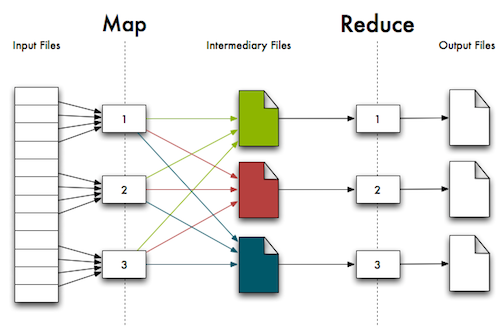
\includegraphics[width=0.8\textwidth]{mapreduce.png}
\caption{Die zwei Phasen eines MapReduce-Jobs \protect\cite{GARFINKEL}}
\end{figure}

\subsection{Open Source}
Googles Implementierung des MapReduce-Frameworks ist nicht öffentlich verfügbar. Die Apache Software Foundation hat sich mit dem Hadoop-Projekt zum Ziel gesetzt ein freies MapReduce-Ecosystem zu entwickeln.

\newpage

\nocite{GFS}
\nocite{GOOGLE-TENZING}
\nocite{GOOGLE-MAPREDUCE}
\nocite{GOOGLE-GFS}
\nocite{KemperEickler}
\nocite{KandziaKlein}
\nocite{Codd}
\nocite{Selinger}
\nocite{Zeller}
\nocite{Ioannidis}
\addcontentsline{toc}{section}{Literatur}
\printbibliography

\newpage

\addcontentsline{toc}{section}{Abbildungsverzeichnis}
\listoffigures

\addcontentsline{toc}{section}{Tabellenverzeichnis}
\listoftables

\addcontentsline{toc}{section}{Quellcodeverzeichnis}
\renewcommand\listoflistingscaption{Quellcodeverzeichnis}
\listoflistings

\end{document}

